%! Author = mariuszindel
%! Date = 25.01.21




\section{Rauschen}

\subsection{Thermisches Rauschen}
\begin{center}
    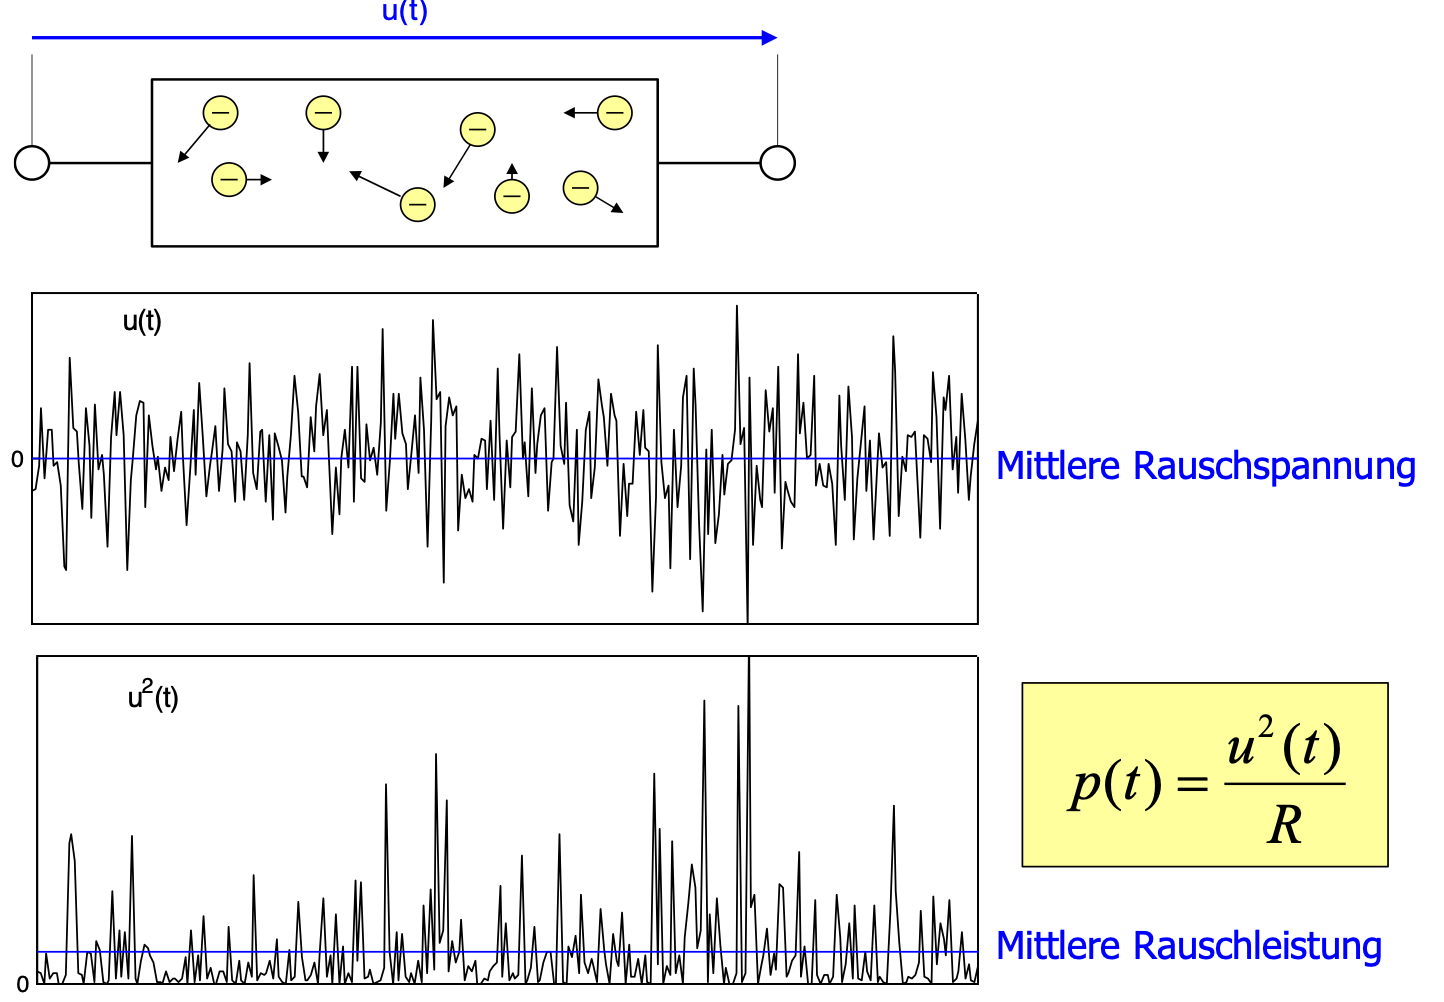
\includegraphics[width=\linewidth]{graphic/rauschen/Thermisches Rauschen.png}
\end{center}
\vspace{-8pt}

\subsubsection{Thermische Rauschleistung}
$N[dBm]=-174dBm+10log_1_0(\Delta f) \\ \Delta f = Frequenzintervall[Hz]$

\textbf{Beispiel:} \\
Systembandbreite = 4GHz
$n=-174dBm+10log_{10}(4*10^9)=-78dBm$\\


\subsection{Weisses Rauschen}
\begin{center}
    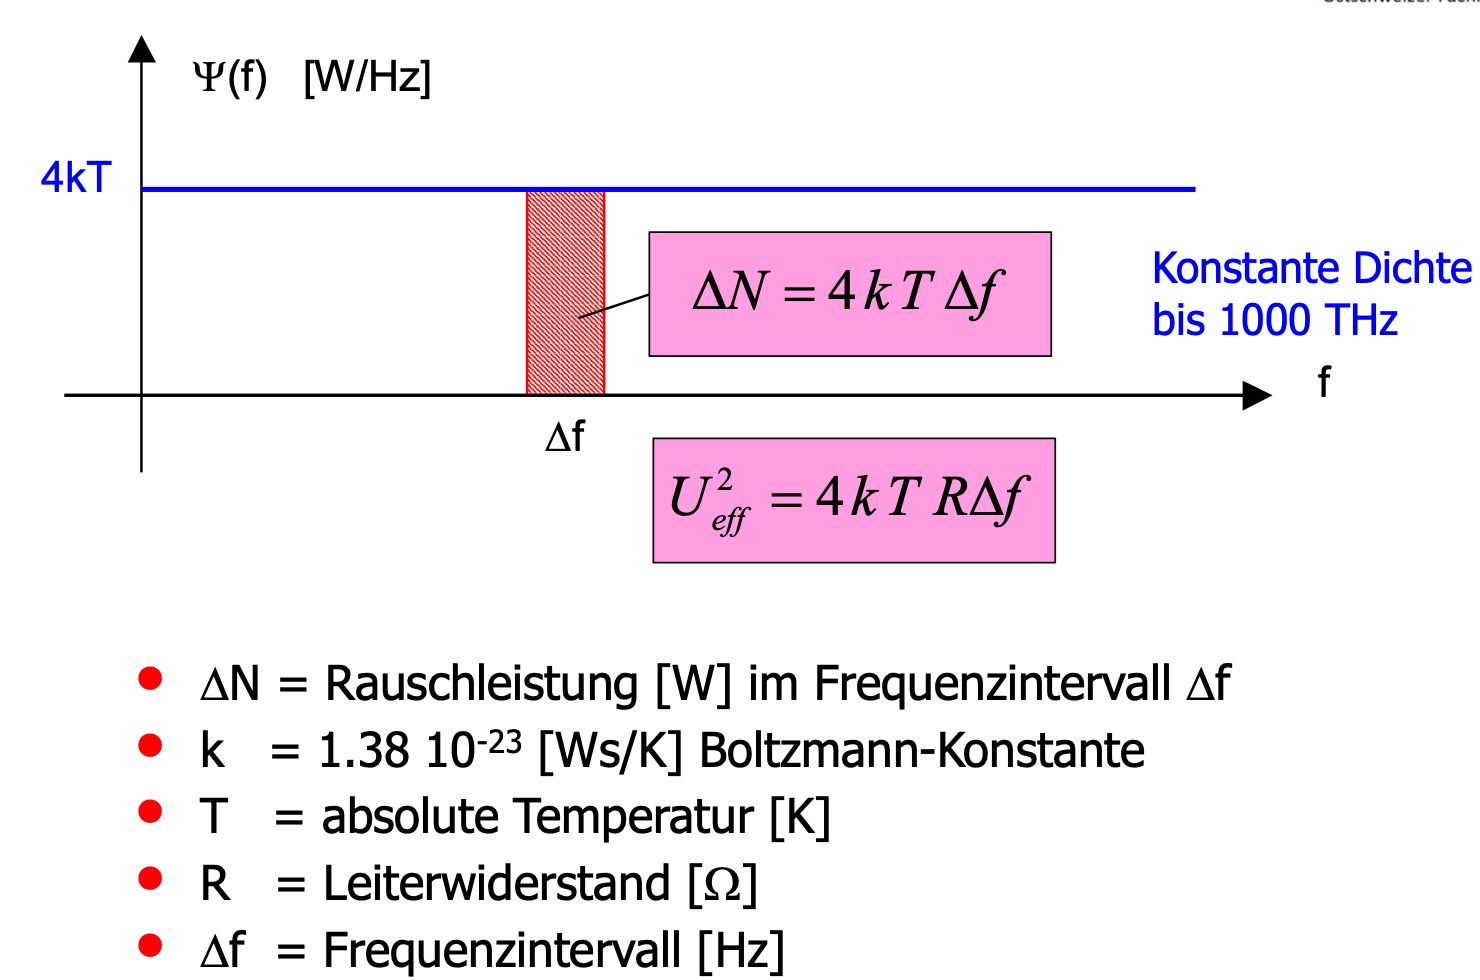
\includegraphics[width=\linewidth]{graphic/rauschen/Weisses Rauschen.png}
\end{center}
\vspace{-8pt}

\subsection{Signal-zu-Rauschverhältnis}
$S / N=\frac{\text { Signalleistung }}{\text { Rauschleistung }}$\\
$=\frac{(\text { Signalamplitude im } \text { Abtastzeitpunkt })^{2}}{(\text { Effektivwert der Rauschspannung })^{2}}$\\
$\mathrm{SNR}=10 \log \mathrm{S} / \mathrm{N} [dB]$